\documentclass[10pt]{beamer}
\usetheme{metropolis}           % Use metropolis theme
\usepackage{graphicx}
\usepackage{amsmath}
\bibliographystyle{IEEEtran}
\title{Machine Learning - Specialized Hardware or Massive Distribution}
\date{\today}
\author{Prajna Kandarpa}
% - Specialized AI Hardware - Google, Intel, NVidia
% - State of Mobile AI models and deployment techniques
% - Federated Learning
% \institute{University of Waterloo}
\begin{document}
\maketitle
\begin{frame}{Overview}
  \tableofcontents
\end{frame}
\section{The State of Machine Learning}
\begin{frame}{History}
  \begin{center}
    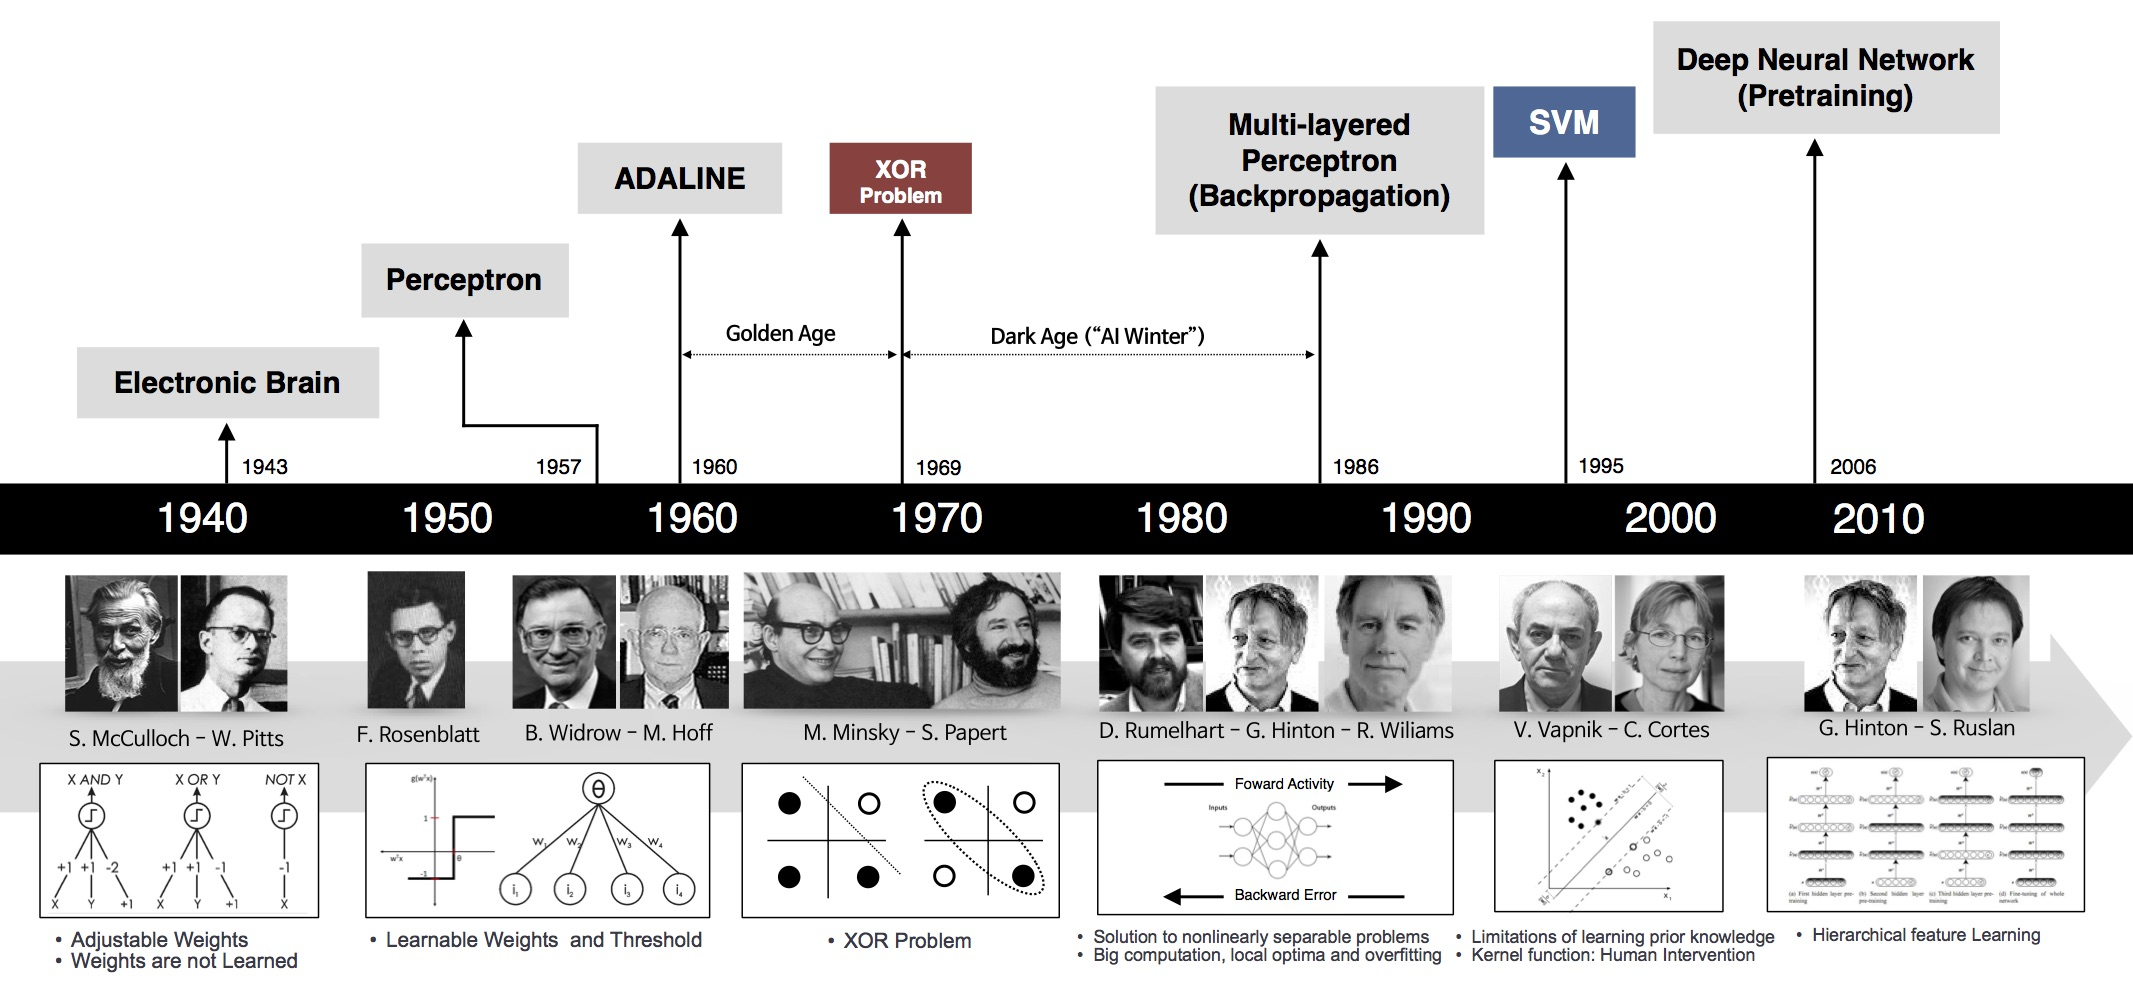
\includegraphics[height=0.4\textwidth]{nn_timeline.jpg}
  \end{center}

  \begin{itemize}
  \item WWII and automatic control systems
  \item Cybernetics Society - Weiner, Mcculloch
  \item Rosenblatt's Perceptron\cite{DeepLear69:online}
  \item Minsky's brutal destruction of the perceptron
  \item AI Winter
  \end{itemize}
\end{frame}
\begin{frame}{Advent of deep learning in 2010}
  \begin{itemize}
  \item Geoff Hinton - Pulled Neural Nets back to mainstream
  \item Had been doing NN research since 1976 - backpropagating errors to learn representations\cite{rumelhart1988learning}
  \item Convnets - Yann LeCunn, AT\&T Bell Labs
  \item Major breakthrough - 2012 - ImageNet competition won by AlexNet
  \end{itemize}
\end{frame}
\begin{frame}{Nvidia and CUDA}
  \begin{figure}
    \centering
    \begin{minipage}{.5\textwidth}
      \centering
      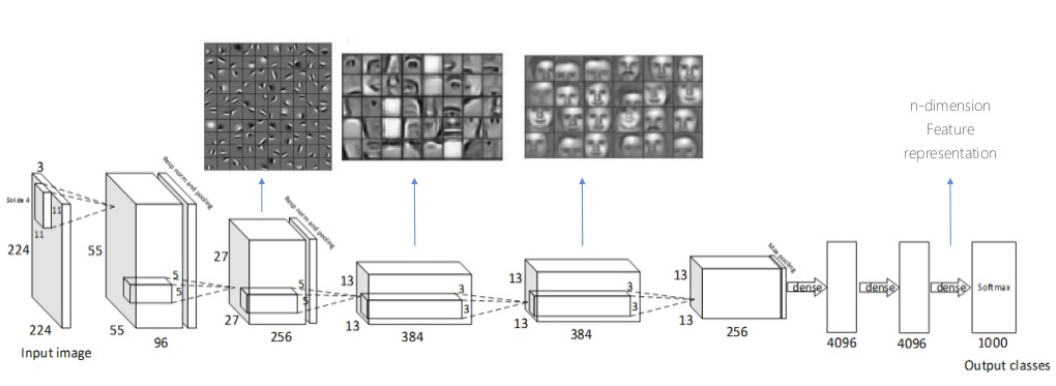
\includegraphics[width=\linewidth]{alexnet.png}
      \label{fig:test1}
    \end{minipage}%
    \begin{minipage}{.5\textwidth}
      \centering
      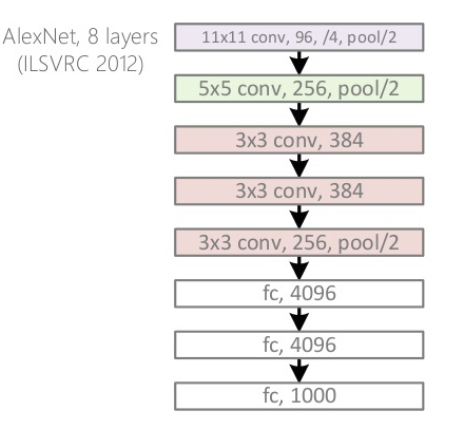
\includegraphics[width=.6\linewidth]{alexnet2.png}
      \label{fig:test2}
    \end{minipage}
    \caption{Alexnet Architecture \cite{krizhevsky2012imagenet}}
  \end{figure}
  \begin{itemize}
  \item AlexNet used GPUs to speed up model training for a CNN
  \item GPUs are massively parallel floating point calculators
  \item Massive parallelization and accelerated memory access
  \item CUDA - parallel computing platform - C, C++ and Fortran
  \item Deep learning computations are matrix operations (multiplications and factorizations)
  \end{itemize}
\end{frame}
\section{AI Accelerators}
\begin{frame}{Facebook - GPU Servers}
  \href{https://www.youtube.com/watch?v=-CRJLam3BNc}{Facebook Artificial Intelligence Research Lab}
  \begin{itemize}
  \item 8 NVIDIA Tesla P100 SXM2 GPUs
  \item High speed data transfers through PCIE slots
  \item 9-18 teraflops per GPU
  \item Not commercially available
  \end{itemize}
\end{frame}
\begin{frame}{Google TPU}
  \begin{center}
    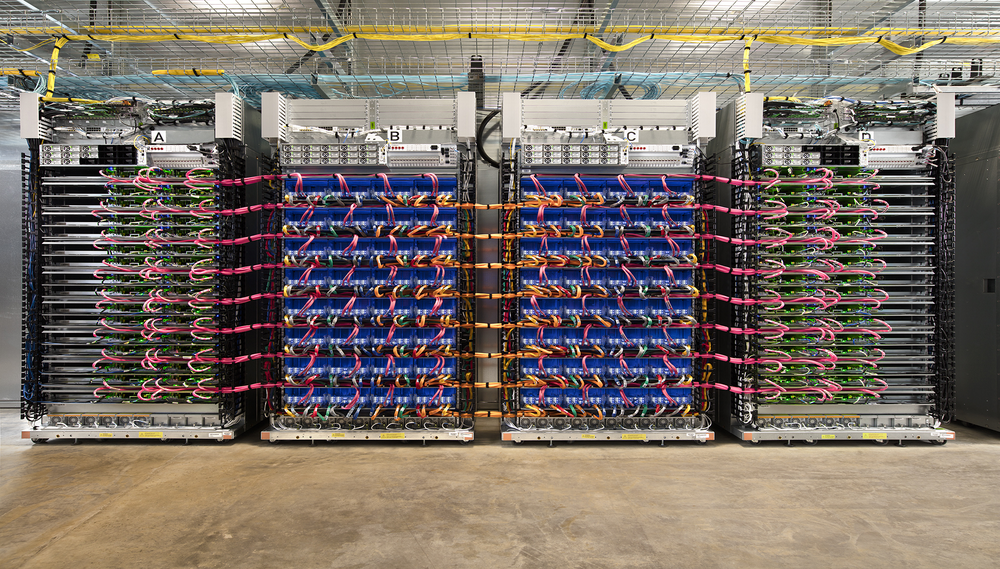
\includegraphics[width=0.45\textwidth]{tpu.png}
  \end{center}
  \begin{itemize}
  \item \href{https://www.youtube.com/watch?v=TnUYcTuZJpM}{Google DeepMind}
  \item \href{https://www.theverge.com/2017/5/17/15649628/google-tensor-processing-unit-tensorflow-ai-training-system}{Google TPU and AI Vision}
  \item Cloud TPUs offer 11.5 petaflops performance
  \item Each Cloud TPU contains 64 TPU units
  \item 25\% increase in performance compared to best GPUs
  \end{itemize}
\end{frame}
\begin{frame}{Intel}
  \begin{itemize}
  \item Nervana Engine - Enterprise compute platform
  \item 8 Tb/s Memory access speeds
  \item FPGAs (from Altera acquisition) for AI compute
  \item \href{https://www.youtube.com/watch?v=hX0UELNRR1I}{Movidius - VPU - focus on drone market, low power}
  \end{itemize}
\end{frame}
\section{ML on mobile devices}
\begin{frame}{Status Quo}
  \begin{center}
    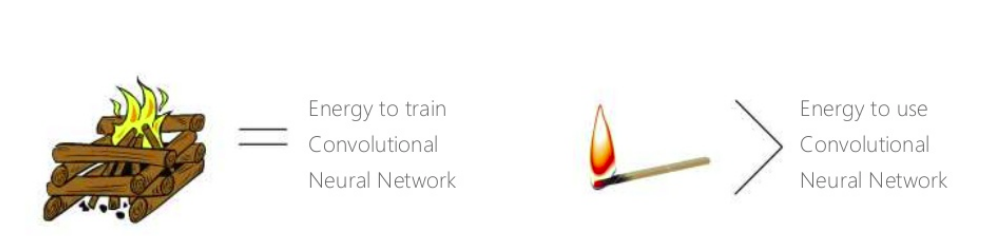
\includegraphics[height=0.23\textwidth]{cnn_energy.png}
  \end{center}
  \begin{itemize}
  \item Pretrained Models and inference engines on device
  \item Frameworks - Tensorflow, Apple CoreML, Torch, Caffe
  \item On Device training on full dataset is unfeasible
  \item Tremendous amount of data collected every second
  \end{itemize}
\end{frame}
\begin{frame}{Decentralized Training}
  \begin{center}
    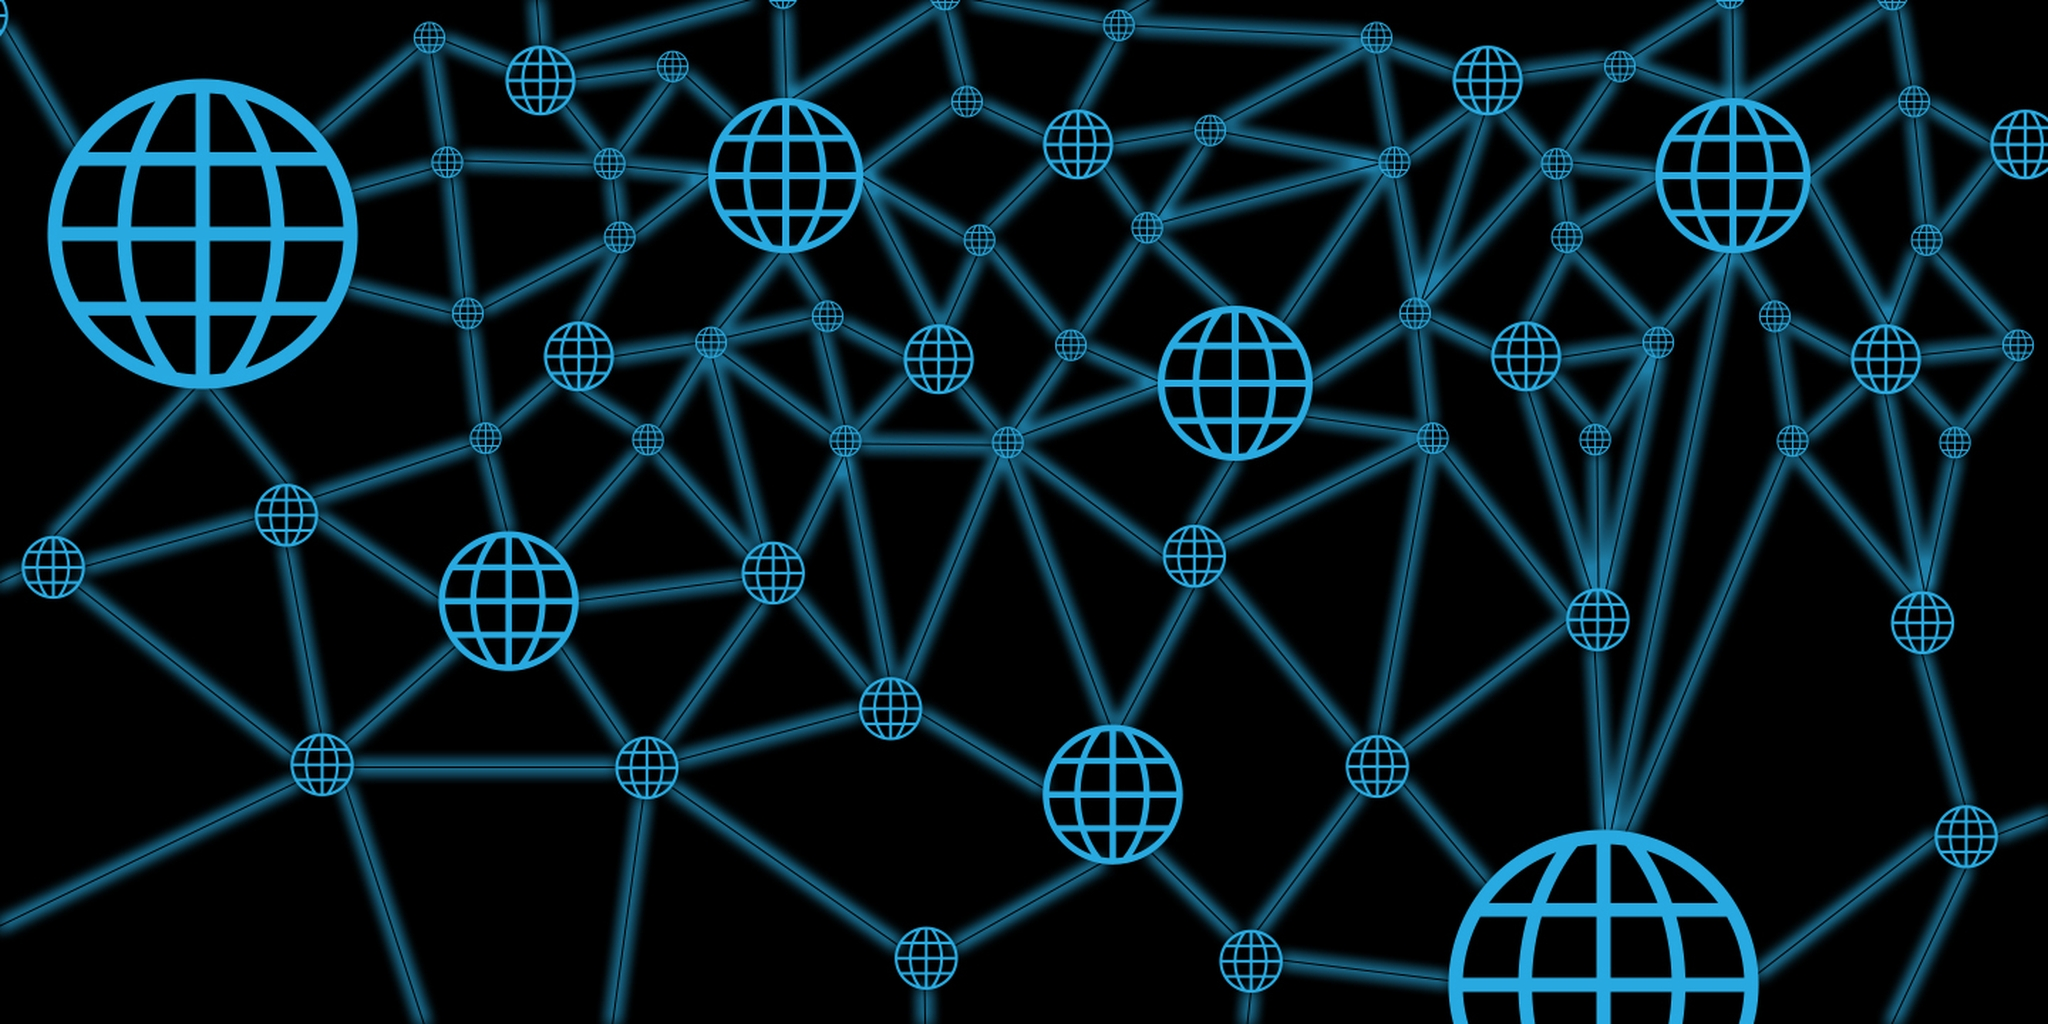
\includegraphics[height=0.4\textwidth]{decent.jpg}
  \end{center}
  \begin{itemize}
  \item Important advances made by Google in distributed training
  \item Isn't everything already distributed ??? - MapReduce, Spark etc.
  \item Make it even more distributed!! - millions of nodes
  \item Sometimes number of nodes exceeds number of training samples
  \end{itemize}
\end{frame}
\begin{frame}{Consequences of Decentralized training}
  \textbf{BAD}
  \begin{itemize}
  \item Training batches not representative of population distribution
  \item Current gradient descent algorithms don't work.
  \end{itemize}
  \textbf{GOOD}
  \begin{itemize}
  \item Less frequent data transfer/retrieval to servers
  \item Increased user privacy due to lesser data transfer
  \end{itemize}
\end{frame}
\section{Federated training and optmization}
\begin{frame}{Federated optimization}
  \begin{center}
    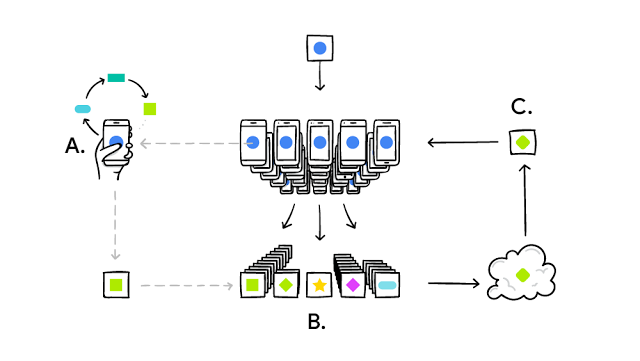
\includegraphics[height=0.4\textwidth]{feder.png}
  \end{center}
  \begin{itemize}
  \item Training Data stays on mobiles
  \item Global model updates from local model update averages
  \item Collect model updates not training samples
  \end{itemize}
\end{frame}
\begin{frame}{Communication Efficiency}
  \begin{itemize}
  \item Data transfer internally much less expensive than external transfers
  \item Inter node communication dominates training times
  \item Fed Learn. reduces communication times to once per day between a node
    and server
  \end{itemize}
\end{frame}

\begin{frame}{Federated Stochastic variance Reduced Gradient}
  \begin{itemize}
  \item Uses SVRG for countering the effects of non IID data by explicit
    variance reduction\cite{DBLP:journals/corr/KonecnyMRR16}
  \end{itemize}
  \textbf{DANE (Distributed Approximate Newton Algorithm)}
  \begin{itemize}
  \item Estimates the empirical loss function via convex combination of local
    loss functions
  \item Form local subproblems, dependent on local data and can converge in O(1)
    rounds of communication
  \end{itemize}

\end{frame}
\section{Performance Comparisons}
\begin{frame}{Predicting comments on Google+ posts}
  \begin{center}
    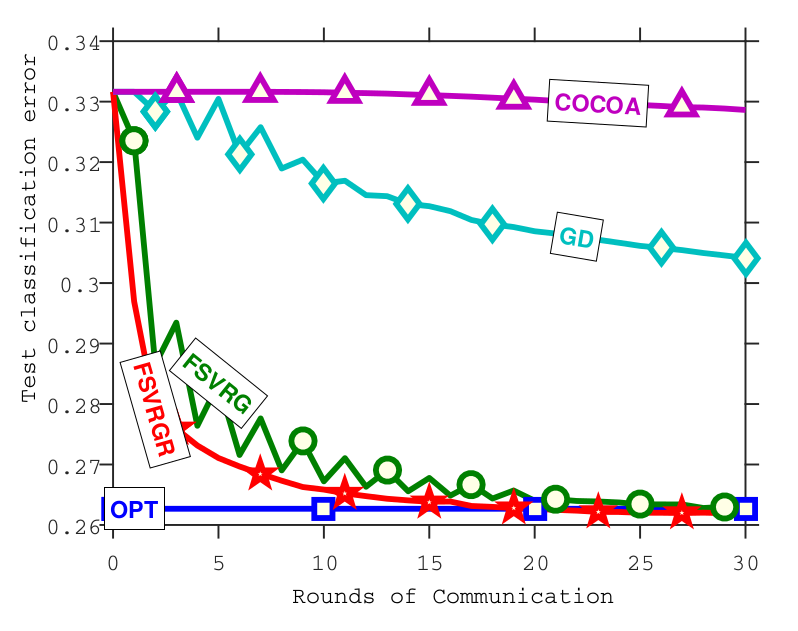
\includegraphics[height=0.7\textwidth]{fedsvrg.png}
  \end{center}

\end{frame}
\section{AL acceleration v/s Large scale distribution}
\begin{frame}{Privacy implications}
  \begin{itemize}
  \item Secure aggregation of user data
  \item enable differential privacy to an extent
  \item only offered by federated learning unless
  \item Cloud ML providers get better at implementing differential privacy
  \end{itemize}
\end{frame}
\begin{frame}{Cost Benefits}
\end{frame}
\begin{frame}{References}
  % \te
  \bibliography{presentation}
\end{frame}
\end{document}